% !TEX encoding = UTF-8 Unicode
\documentclass[12pt]{article}

% Pacotes %
\usepackage[brazilian]{babel}
\usepackage[utf8]{inputenc}
\usepackage[T1]{fontenc}
\usepackage{amsmath}
\usepackage{enumitem}
\usepackage{hyperref}
\usepackage{graphicx}
\usepackage{verbatimbox}

% Definições de titulo e autores %
\title{Iniciação a Computação Científica\\Trabalho 2}
\author{
	Giancarlo Klemm Camilo \\
	Renan Domingos Merlin Greca
}
\date{Junho de 2015}

% Inicio do documento %
\begin{document}

% ------------------------------------------------------ %
% Página inicial %
\maketitle
\newpage	

% ------------------------------------------------------ %
% Indice %
\tableofcontents
\newpage

% ------------------------------------------------------ %
\section{Introdução}
O objetivo deste trabalho é a implementação de programa para resolver o PDE:

...

Após o programa inicial foi feito, várias alterações foram feitas para melhorar o desempenho. Os métodos utilizados para análise do código, sistema de testes, otimizações de código e de estruturas de dados são descritas nas seções seguintes.

\newpage

% ------------------------------------------------------ %
\section{Análise de Arquitetura}
\paragraph{}
A máquina escolhida para testes foi a achel do departamento de informática da UFPR.

\subsection{Topologia dos Processadores}
\paragraph{Tipo do CPU} Intel Core Westmere processor
\paragraph{Número de processadores} 2
\paragraph{Núcleos} 12

\subsection{Topografia de Cache}
\paragraph{Level 1} 32kB por núcleo
\paragraph{Level 2} 256kB por núcleo
\paragraph{Level 3} 12MB por processador

\subsection{Memória}
24GB por processador

\newpage

% ------------------------------------------------------ %
\section{Limite Superior da Discretização}

\begin{align}
	T &\cong n_x + 1 = n_y + 1 \\
	|X| &= (n_x+1)\times(n_y+1)\times8 bytes \cong T^2\times8 bytes \\
	|B| &= (n_x+1)\times(n_y+1)\times8 bytes \cong T^2\times8 bytes \\
	|R| &= (n_x+1)\times(n_y+1)\times8 bytes \cong T^2\times8 bytes \\
	|X| + |B| + |R| &= 24000000 \\
	3\times T^2\times8 &= 24000000 \\
	T^2 &= 3000000\\
	T &\cong 1732
\end{align}

\paragraph{}
A nova versão do programa aceita valores de até aproximadamente 1.732 para $n_y$ e $n_x$ numa máquina com 24GB de RAM e desconsiderando o uso de memória virtual.
Ou seja, pode computar até 3.000.000 de pontos.

\newpage

% ------------------------------------------------------ %
\section{Tempo de Execução}

	\subsection{Programa Original}
	

	\subsection{Programa Otimizado}
	\begin{figure}[ht!]
		\centering
		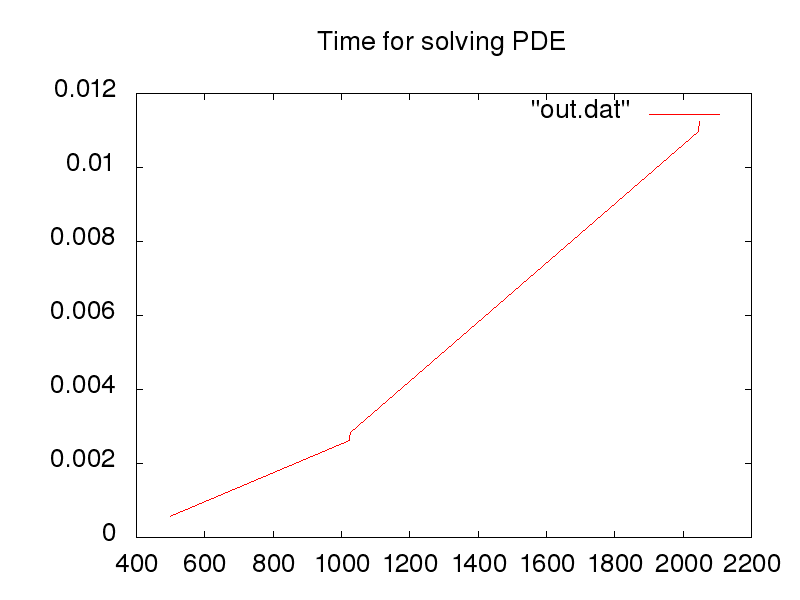
\includegraphics[width=90mm]{newtime.png}
		\caption{Tempo para N\{x,y\} = \{500, 512, 1022, 1024, 1026, 2046, 2048\} 			\label{overflow}}
	\end{figure}
\newpage

% ------------------------------------------------------ %
\section{Análise de Funções}

	\subsection{Programa Original}
		\subsubsection{Método de Gauss-Seidel}
		\subsubsection{Cálculo do Resíduo}
	
	\subsection{Programa Otimizado}
		\subsubsection{Método de Gauss-Seidel}
		\subsubsection{Cálculo do Resíduo}

	\subsection{Análise dos Dados}

\newpage

% ------------------------------------------------------ %
\section{Otimização do Ponto de Interesse}

\paragraph{}
O ponto de interesse escolhido foi o cálculo do vetor $x$ no método de Gauss-Seidel.
Para isso, otimizações foram feitas nas estruturas de dados usadas durante o cálculo e na estrutura do laço em si.

	\subsection{Estrutura de dados}
	\paragraph{}
	A estrutura de dados que mais sofreu alterações foi a matriz $A$.
	Na versão original do programa, $A$ tinha o tamanho de $((n_x+1)\times(n_y+1))^2$, representando a matriz inteira do método analítico de Gauss Seidel.
	
	Olhando para a matriz $A$, percebemos que grande parte das posições tinham valor $0$ e que os valores de interesse de cada linha estavam numa distância de $(n_y+1)$ da diagonal principal da matriz.
	Ou seja, os dados que estavam além desse intervalo eram sempre $0$ e poderiam ser ignorados.
	
	Além disso, percebemos que as posições ao redor da diagonal principal sempre seguiam o seguinte padrão:
	
	\begin{center}
		\texttt{$h_x$ 0 $h_y$ 1 $h_y$ 0 $h_x$}
	\end{center}
	
	Onde o elemento na diagonal principal é sempre $1$, $h_x$ e $h_y$ representam a dependência dos pontos adjacentes e, no exemplo acima, $n_y=2$.
	Sendo assim, podíamos ignorar as posições que sempre continham $1$ ou $0$, além de evitar a repetição de $h_x$ e $h_y$.
	
	Também foi possível ver que os valores de $h_x$ e $h_y$ permaneciam constantes em quase todas as linhas da matriz, exceto nas linhas em que não estavam presentes.
	As linhas que não continham $h_x$ e $h_y$ representavam os pontos das bordas da grade, que são calculadas separadamente.
	Logo, foi possível ver que uma matriz que simplesmente nos dizia se um determinado ponto é ou não uma borda era suficiente para fazer os cálculos de Gauss-Seidel, se salvássemos $h_x$ e $h_y$ em variáveis separadas.
	
	Portanto, na versão atual, a matriz $A$ tem o tamanho de $(n_x+1)\times(n_y+1)$ e utiliza o tipo de dados \emph{short int}, pois apenas armazenamos $0$ quando o ponto é uma borda ou $1$ caso contrário.

	\subsection{Código}
	
	Na versão anterior do programa, o laço de Gauss-Seidel continha quatro desvios condicionais, um para cada borda.
	Nesta versão, temos apenas um desvio que utiliza a matriz $A$ para verificar se o ponto em questão é borda ou não.
	
	Caso o ponto não seja uma borda, quatro operações são realizadas utilizando os valores de $h_x$ e $h_y$ e outras posições do vetor $x$.
	Na versão original do programa, as quatro operações eram armazenadas na variável \texttt{temp} utilizando o operador \texttt{+=}.
	Isso causava problemas no pipeline da execução, pois gerava uma dependência de dados onde todas as operações em ponto flutuante da linha anterior precisavam ser computadas antes do início dos cálculos da próxima.

\newpage

% ------------------------------------------------------ %
% Resultados %
\section{Resultados}

\subsection{Tempo}

\subsection{Memória}

\newpage

\end{document}